% add the answers flag to print the solutions.
\documentclass[addpoints, answers]{exam}

\usepackage[utf8]{inputenc}
\usepackage{calc}
\usepackage[dvipsnames]{xcolor}
\usepackage{ifthen}
\usepackage{tcolorbox}

% \makebox[\textwidth]{Name:\enspace\hrulefill}
%  
% \vspace{5mm}
%\makebox[\textwidth]{Instructor’s name:\enspace\hrulefill}

\definecolor{MyLightGray}{gray}{0.60}

\newcommand{\truefalse}
{		\begin{checkboxes}
			 \choice True
			 \choice False. Explanation: 
		\end{checkboxes}
		\vspace{10pt}
}


% Check if 'answers' is an option
\newcommand{\ifanswers}[2]{%
  \ifthenelse{\boolean{exam@answers}}{#1}{#2}%
}



\newcommand{\answerspace}[1]
{
	\ifprintanswers
	\else
		\setlength{\mylength}{10pt}%
		% \vspace{#1\mylength}
		% Make the grey box
		\par\nobreak\noindent
		\makebox[\linewidth][l]{%
			% set inner padding to zero, so only the frame shows
			{\setlength{\fboxsep}{0pt}%
			% draw a color frame, white (or transparent) inside
			\fcolorbox{MyLightGray}{white}{%
			% the inner box has zero width content but fixed height
			\parbox[t][#1\mylength][c]{%
				% subtract twice the frame‐thickness from the full width
				\dimexpr\linewidth-2\fboxrule\relax
			}{\strut}%
			}%
			}%
		}%
		\par
		\vspace{3\mylength}

  	\fi
}
\newlength{\mylength}

\newcommand{\code}[1]{{\texttt{#1}}}

\newcommand{\answer}[1]{\begin{solution}{#1}\end{solution}}




%\usepackage{listings}
\usepackage{color}
\usepackage{lastpage}
\usepackage{verbatim}
\usepackage{fancyvrb}
\usepackage{graphicx}
\usepackage{float}
\usepackage{minted}
\usepackage{multicol}

\newcommand{\includecode}[2][c]{\lstinputlisting[caption=, escapechar=, language=#1]{#2}}
\RecustomVerbatimCommand{\VerbatimInput}{VerbatimInput}{}

\newcommand{\Code}[1]{\mintinline{python}{#1}}
% x, a, b, y  --- the four inputs to the predicate in Q9.
\newcommand{\ACC}[4]{\Code{bar(#1, #2, #3, #4)}}

\renewcommand{\solutiontitle}{\noindent\textbf{Solution sketch: }}

\definecolor{SolutionColor}{rgb}{0.8,0.9,1}

\cfoot{Page \thepage\ of \pageref{LastPage}}

\rhead{Initials: \rule{20mm}{0.4pt}}


%%%%%%%%%%%%%%%%%%%%%%%%%%%%%%%%%%%%%%%%
\begin{document}
\fvset{numbers=left,numbersep=3pt}
\thispagestyle{empty}

\begin{center}
	{\LARGE CS 408 Fall 2026 -- Practice Midterm 1 \\}
\vspace{.5in}


\fbox{\fbox{\parbox{5.5in}{\centering
	\begin{itemize}
        \item We have deliberately made this practice midterm harder,
          more open-ended, and longer than the actual midterm, since
          there are no time constraints (and the course staff is not
          on the hook for grading your answers :)). \textbf{The goal
            here is to help you study}: if you can ace the practice
          midterm, you should have no problem with the real
          deal. Thus, while we will provide you with solutions next
          week, you should try to answer all these questions on your
          own, before consulting our answers.

        \item Try to be concise: when a question asks for an
          explanation, a few sentences should suffice. Aim for
          quality, not quantity!

        \item Show enough of your reasoning so that we can award
          partial credit for a correct approach.

        \item Answer the questions in the spaces provided. Your answer
          does not need to take up all the space provided (hopefully
          we've given you more than enough room!). If you do run out
          of space, make a note and then use the empty pages at the
          back of the exam to complete your answer. Be sure to clearly
          label any answers on those pages with the corresponding
          question.

        \item Several questions ask you to provide something ``if
          possible.'' If it is not possible, you should plainly say so
          and then explain why that is the case.

        \item Coding questions should be answered in Python, unless
          stated otherwise.

        \item Unless otherwise noted, CFG nodes represent basic
          blocks. When necessary, refer to nodes using the labels
          given in the figure.

        \item Please double check that your copy of the exam
          is complete; you should have \pageref{LastPage}
          pages.

        \item You have 75 minutes to complete the exam.
        \end{itemize}
	}}}
\end{center}

\vspace{5mm}
\begin{center}
	\makebox[0.6\textwidth]{
		\combinedgradetable[h][questions]
	}
\end{center}

\begin{questions}

\newpage

% ========================================================
% Q1: faults, errors, failures.  [sample-midterm Q1]
% ========================================================

\question Consider the concepts of faults, errors, and failures.

\begin{parts}

\part[3] What is the difference between an error state and a failure?
  Explain. %
  \answerspace{9} %
  \begin{solution} %
    An error state is an \textit{incorrect internal state of the
      program}, e.g.\ when an internal variable holds a value it would
    never hold if the program did not contain a fault.

    A failure is an observable behavior that is inconsistent with the
    expected behavior: the program crashes when it should not, or it
    produces the wrong output. %
  \end{solution}

\part[3] What is the relationship between an error state and a
  failure? Explain. %
  \answerspace{10} %
  \begin{solution} %
    A program \textbf{must} encounter an error state in order for a
    failure to happen. Put another way, an error state is a
    \textit{necessary precondition} for a failure. \\

    Importantly, however, not all error states lead to failures. %
  \end{solution}

\end{parts}

% ========================================================
% Q2: three approaches + ISP.  [sample-midterm Q2]
% ========================================================

\question Consider the following three approaches to testing a function:
  \begin{itemize}
  \item \textbf{Approach 1:} Run the target program on $N$ randomly
    chosen inputs
  \item \textbf{Approach 2:} Run the target program on a
    representative set of $N$ inputs
  \item \textbf{Approach 3:} Run the target program on all inputs
  \end{itemize}
  You can assume $N$ is on the order of tens of thousands.

\begin{parts}

\part[3] Explain the pros and cons of the first ($N$ random inputs) and
  last (all inputs) approaches. %
  \answerspace{11}%
  \begin{solution}%
    \begin{itemize}
    \item Approach 1:
      \begin{itemize}
      \item \textbf{Pros:} Simple and efficient; there is a non-zero
        probability of finding failures if they exist.
      \item \textbf{Cons:} The likelihood of finding errors is
        proportional to the size of the input space and becomes
        vanishingly small as the total number of possible inputs
        grows. A purely random selection strategy is likely to miss
        corner cases.
      \end{itemize}
    \item Approach 3:
      \begin{itemize}
      \item \textbf{Pros:} Comprehensive; will eventually find every
        fault that exists (assuming the function terminates on all
        inputs).
      \item \textbf{Cons:} Testing is unlikely to finish within the
        heat death of the universe.
      \end{itemize}
    \end{itemize}
  \end{solution}

\part[3] Describe how a tester might use input space partitioning to
  identify a ``representative set of inputs'' used by the second
  approach. %
  \answerspace{9}%
  \begin{solution}%
    A tester partitions the set of inputs into equivalence classes and
    selects a representative input from each class.

    Inputs in the same class are expected to behave similarly, while
    inputs in different classes are expected to behave differently.
  \end{solution}

\part[3] What is the main advantage of the last approach over the other
  two? %
  \answerspace{9} %
  \begin{solution}%
    The main advantage of the third approach is that it is
    \emph{complete} --- since it is exhaustive, if a failure exists it
    will be found. Conversely, if exhaustive testing does not discover
    a failure, the function is guaranteed to behave correctly.

    In contrast, the other approaches are sampling techniques, and can
    only guarantee the absence or presence of failures on the inputs
    they have examined. %
  \end{solution}

\end{parts}

\newpage

% ========================================================
% Q3: CFGs and basic blocks.  [sample-midterm Q3]
% ========================================================

\question Consider the following function:
  \begin{minted}{python}
def binary_search(arr: list[int], x: int) -> int:
    l = 0
    r = len(arr) - 1
    while l <= r:
        mid = l + (r - l) // 2
        if arr[mid] == x:
            return mid
        if arr[mid] < x:
            l = mid + 1
        else:
            r = mid - 1
    return -1   # element not found
\end{minted}

\begin{parts}

\part[4] Draw the CFG of this program. Label each node with the basic
  block it represents. Use a range of line numbers when necessary,
  e.g.\ use BB2-7 as the label for a basic block starting at line 2
  and ending at line 7. %
  \answerspace{22} %
  \begin{solution} %
      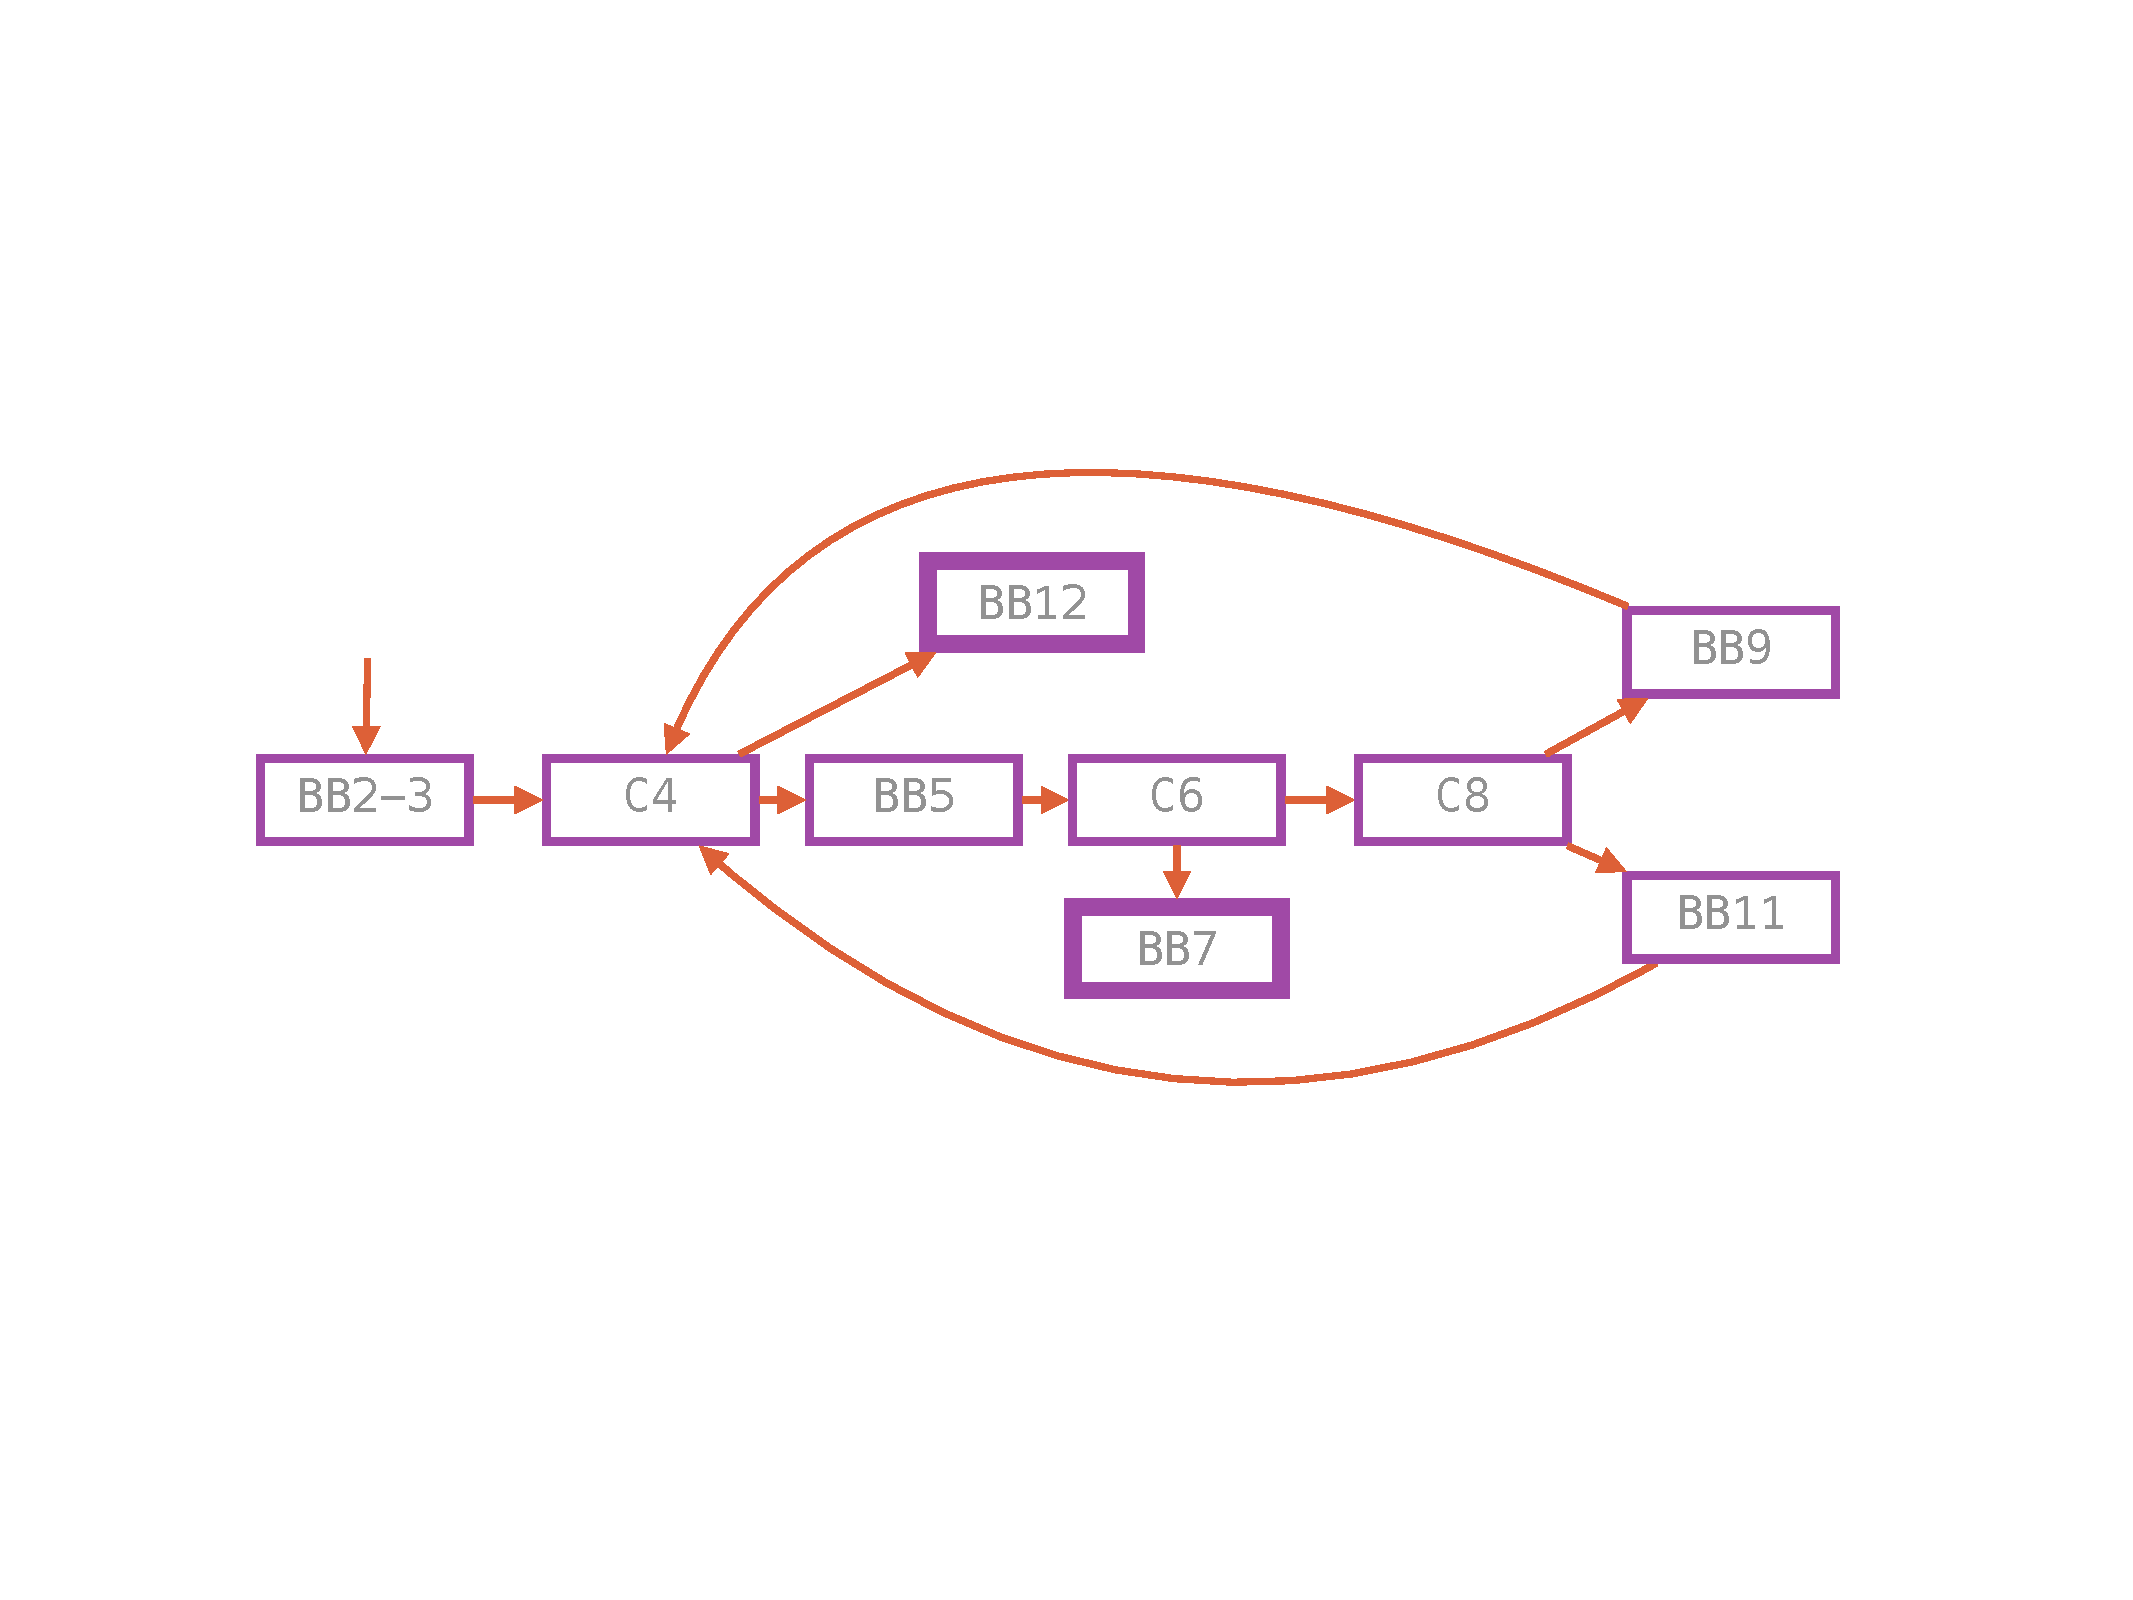
\includegraphics[width=.75\linewidth]{figures/sample-midterm-binary-search-cfg.pdf}
  \end{solution}

\part[3] What is a basic block? %
  \answerspace{9} %
  \begin{solution} %
    A basic block is a sequence of consecutive statements with one
    entry point and one exit point, with no jump into or out of the
    middle.
  \end{solution}

\part[2] Is there any advantage to using basic blocks as opposed to
  statements in CFGs? %
  \answerspace{9} %
  \begin{solution} %
    Yes. It creates a much more compact graph, which is more efficient
    for most program analyses. %
  \end{solution}

\part[2] Is there any disadvantage to using basic blocks as opposed to
  single statements in CFGs? %
  \answerspace{9} %
  \begin{solution} %
    For structural coverage analysis there is generally no
    disadvantage. (Other answers are also valid if well justified ---
    e.g.\ it is harder to talk about the program state \emph{between}
    two statements that live in the same block, which matters for
    data-flow analysis.)
  \end{solution}

\end{parts}

\newpage

% ========================================================
% Q4: RIPR on a faulty program.  [sample-midterm Q4]
% ========================================================

\question Consider the following Python function:
  \begin{minted}{python}
def index_even(x: list[int], n: int) -> int:
    # if x is None, return -1
    # otherwise return the index of the n-th even number in list x,
    # so that n=1 returns the first even element, n=2 the second,
    # *or* return -1 if there is no n-th even number in x
    if x is None:
        return -1
    count = 0
    for i in range(len(x)):
        if x[i] % 2 == 0:
            if count == n:
                return i
            else:
                count += 1
    return -1
\end{minted}

\begin{parts}
\part[3] State the location(s) of the program fault and explain how you
  would fix the program. Consider only the smallest and simplest fix. %
  \answerspace{10} %
  \begin{solution} %
    The simplest explanation\footnote{Other answers are also valid if
      well justified.} is that the fault is on line 8. By starting
    \Code{count} at 0, this function returns the $(n+1)$-th even
    element, since the comment says the first even element is the
    $1$-st one. Replace it with \Code{count = 1}.
  \end{solution}

\part[3] If possible, provide an example of a test input that does not
  cause the fault to execute. If this is not possible, explain why. %
  \answerspace{10} %
  \begin{solution} %
    \Code{index_even(None, 1)} returns on line 7 without ever
    executing line 8. %
  \end{solution}

\part[3] If possible, provide an example of a test input that causes
  the fault to execute but no error state to occur. If this is not
  possible, explain why. %
  \answerspace{10} %
  \begin{solution} %
    Not possible. The initial value of \Code{count} in the correct
    implementation is always 1, so executing line 8 always puts the
    program into a state the correct version would never be in. %
  \end{solution}

\part[3] If possible, provide an example of a test input that causes
  the fault to execute and the error state to occur, but no failure to
  occur. If this is not possible, explain why. %
  \answerspace{10} %
  \begin{solution} %
    \Code{index_even([1, 3, 5], 1)}. The fault executes and
    \Code{count} is erroneously 0, but the list has no even elements,
    so the function returns $-1$ as expected. %
  \end{solution}

\part[3] If possible, provide an example of a test input that causes
  the fault to execute and a failure to occur, but no error state to
  occur. If this is not possible, explain why. %
  \answerspace{10} %
  \begin{solution} %
    Impossible: as in Q1(b), an error state \emph{must} be encountered
    in order for a failure to be observed. %
  \end{solution}

\part[4] Describe and explain the condition that an input must satisfy
  for the error state to occur. %
  \answerspace{10} %
  \begin{solution} %
    The error state occurs whenever \Code{x} is not \Code{None}, since
    line 8 will always be reached in that scenario.
  \end{solution}

\part[4] Describe and explain the condition that an input must satisfy
  for the failure to occur. %
  \answerspace{10} %
  \begin{solution} %
    A failure occurs exactly when \Code{x} is not \Code{None} and
    contains \emph{at least} \Code{n} even elements. With fewer than
    \Code{n} evens both versions return $-1$; with at least \Code{n},
    the faulty version returns either the wrong index or $-1$ where an
    index was expected.

  \end{solution}
\end{parts}

\newpage

% ========================================================
% Q5: construct a program failing two criteria.  [sample-midterm Q5]
% ========================================================

\question Write below a single valid Python program with fewer than 12
  lines and 12 statements that for which it is \textbf{impossible} for
  a test set to completely satsify two different coverage criteria
  discussed in class.

  \answerspace{10} %
  \begin{solution} %
    \begin{minipage}{.8\linewidth}
\begin{minted}{python}
def silly_but_fun():
    if False:
        print("Hello World!")
\end{minted}
    \end{minipage}
  \end{solution}

\begin{parts}
\part[3] Identify the first coverage criterion you selected and
  explain in 2-3 sentences why it is impossible for any test suite to
  satisfy it for your program. %
  \answerspace{7} %
  \begin{solution} %
    No test suite can satisfy node coverage for
    \Code{silly_but_fun}: line 3 is dead code and can never be
    reached. %
  \end{solution}

\part[3] Identify the second coverage criterion you selected and
  explain in 2-3 sentences why it is impossible for any test suite to
  satisfy it for your program. %
  \answerspace{7} %
  \begin{solution}%
    No test suite can satisfy edge coverage either, since the true
    branch of the conditional can never be taken. %
  \end{solution}
\end{parts}

\newpage

% ========================================================
% Q6: paths.  [sample-midterm Q6]
% NOTE: needs figures/sample-midterm-cfg-2.pdf (nodes A--E).
% ========================================================

\question Consider the following control-flow graph:
  \begin{center}
    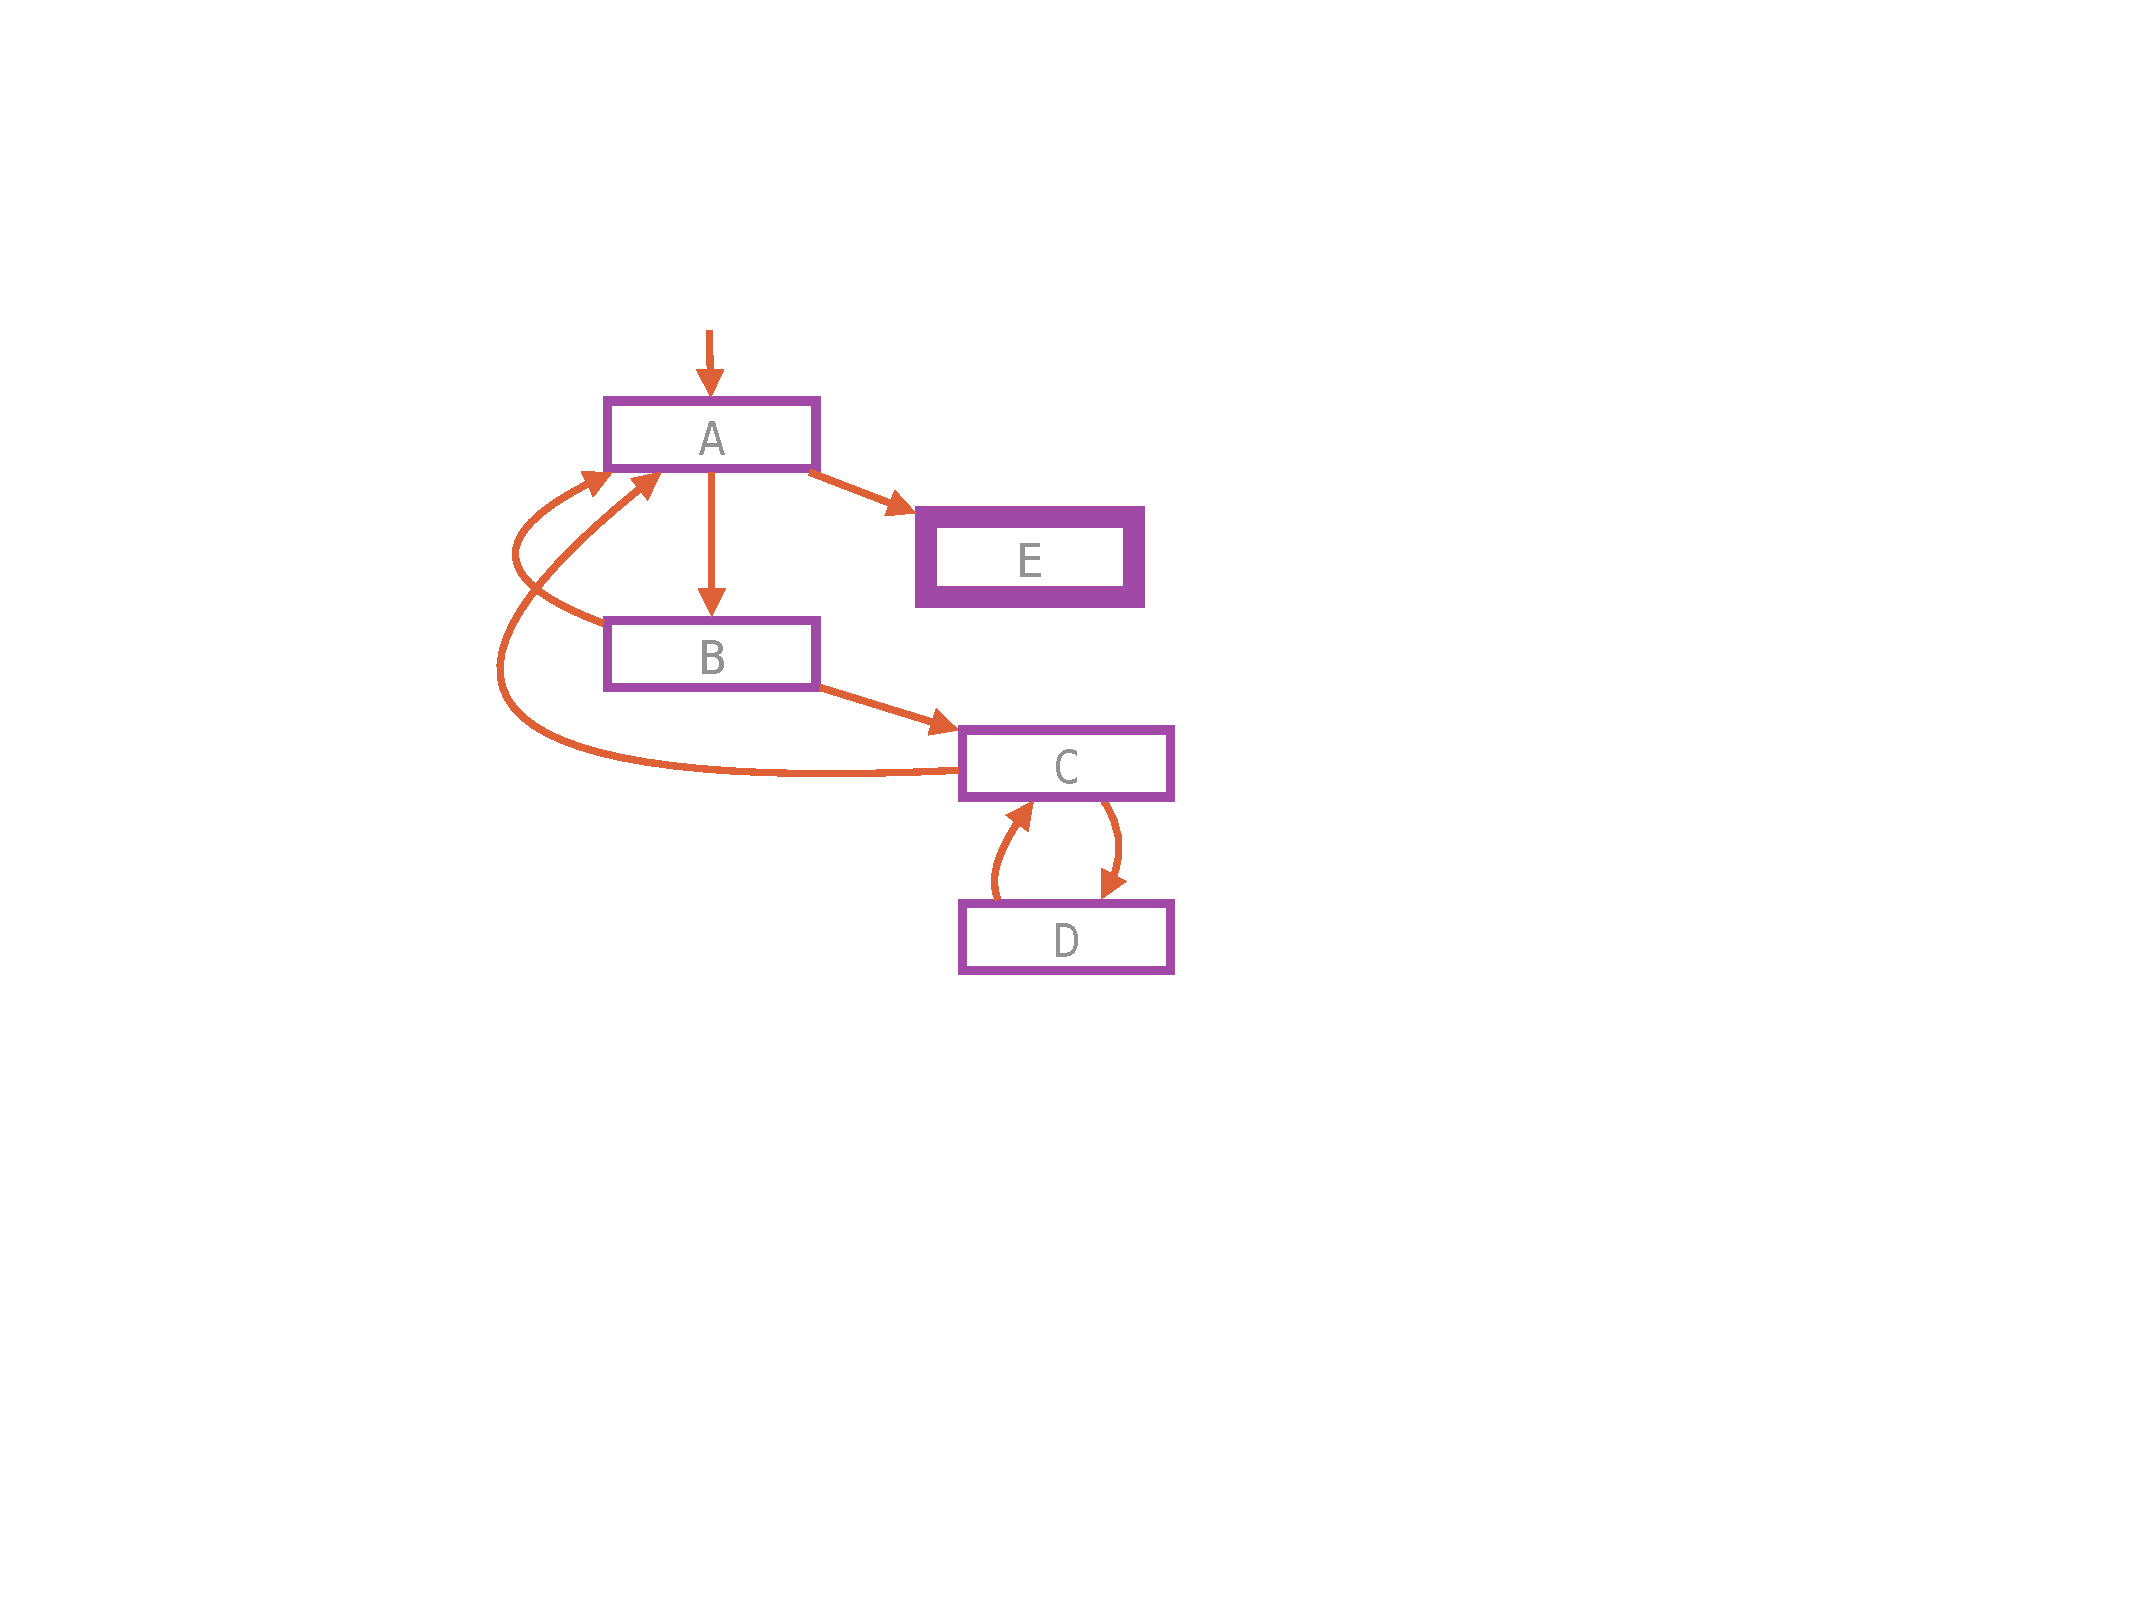
\includegraphics[width=7cm]{figures/sample-midterm-cfg-2.pdf}
\end{center}

\begin{parts}
\part[3] List all the simple paths in the CFG given above. %
  \answerspace{7} %
  \begin{solution} %
    \begin{itemize}
      \item[1] [A], [B], [C], [D], [E]  %
      \item[2] [A, E], [A, B], [B, A], [B, C], [C, A], [C, D], [D, C] %
      \item[3] [A, B, A], [A, B, C], [B, A, B], [B, A, E], [B, C, D],
        [B, C, A], [C, A, B], [C, A, E], [C, D, C], [D, C, A],
        [D, C, D] %
      \item[4] [A, B, C, D], [A, B, C, A], [B, C, A, B], [B, C, A, E],
        [C, A, B, C], [D, C, A, E], [D, C, A, B] %
      \end{itemize}
  \end{solution}

\part[3] List three test paths in the CFG given above. %
  \answerspace{7} %
  \begin{solution} %
    Test paths must start at node A and end at node E. Note that there
    is exactly one \emph{simple} test path: [A, E]. Once you allow
    repeated nodes the world is your oyster: [A, B, A, E],
    [A, B, C, D, C, A, E], and so on.
  \end{solution}

% \part[3] List all the prime paths in the CFG given above. %
%   \answerspace{7} %
%   \begin{solution} %
%     A prime path is a simple path that is not a proper subpath of any
%     other simple path.
%     [A, B, A], [B, A, B], [B, A, E], [C, D, C], [D, C, D],
%     [A, B, C, A], [A, B, C, D], [B, C, A, B], [B, C, A, E],
%     [C, A, B, C], [D, C, A, B], [D, C, A, E]
%   \end{solution}

\newpage
\part[10] Write an example of a syntactically valid Python function
  that generates the control-flow graph above. If this is not
  possible, explain why. %
  \answerspace{23} %
  \begin{solution}
    One possible solution:
\begin{minted}{python}
def silly_and_also_fun(a: int) -> int:
    while a <= 52:          # A
        if a < 53:          # B
            while a < 53:   # C
                a += 1      # D
    return a                # E
\end{minted}
  \end{solution}

\part[3] Provide test inputs that would generate the test paths you
  identified in part (b), or state that they are infeasible. %
  \answerspace{15} %
  \begin{solution}
    \begin{itemize}
    \item[] \textbf{[A, E]}: \Code{silly_and_also_fun(53)}
    \item[] \textbf{[A, B, A, E]}: infeasible
    \item[] \textbf{[A, B, C, D, C, A, E]}: \Code{silly_and_also_fun(52)}
    \end{itemize}
  \end{solution}
\end{parts}

\newpage

% ========================================================
% Q7: data-flow criteria.  [sample-midterm Q7]
% NOTE: needs figures/sample-midterm-cfg.pdf
% ========================================================

\question Consider the following control-flow graph annotated with
  def-use information. Unless otherwise noted, assume $def(l) =
  \emptyset$ and $use(l) = \emptyset$.
  \begin{figure}[ht]
    \begin{center}
      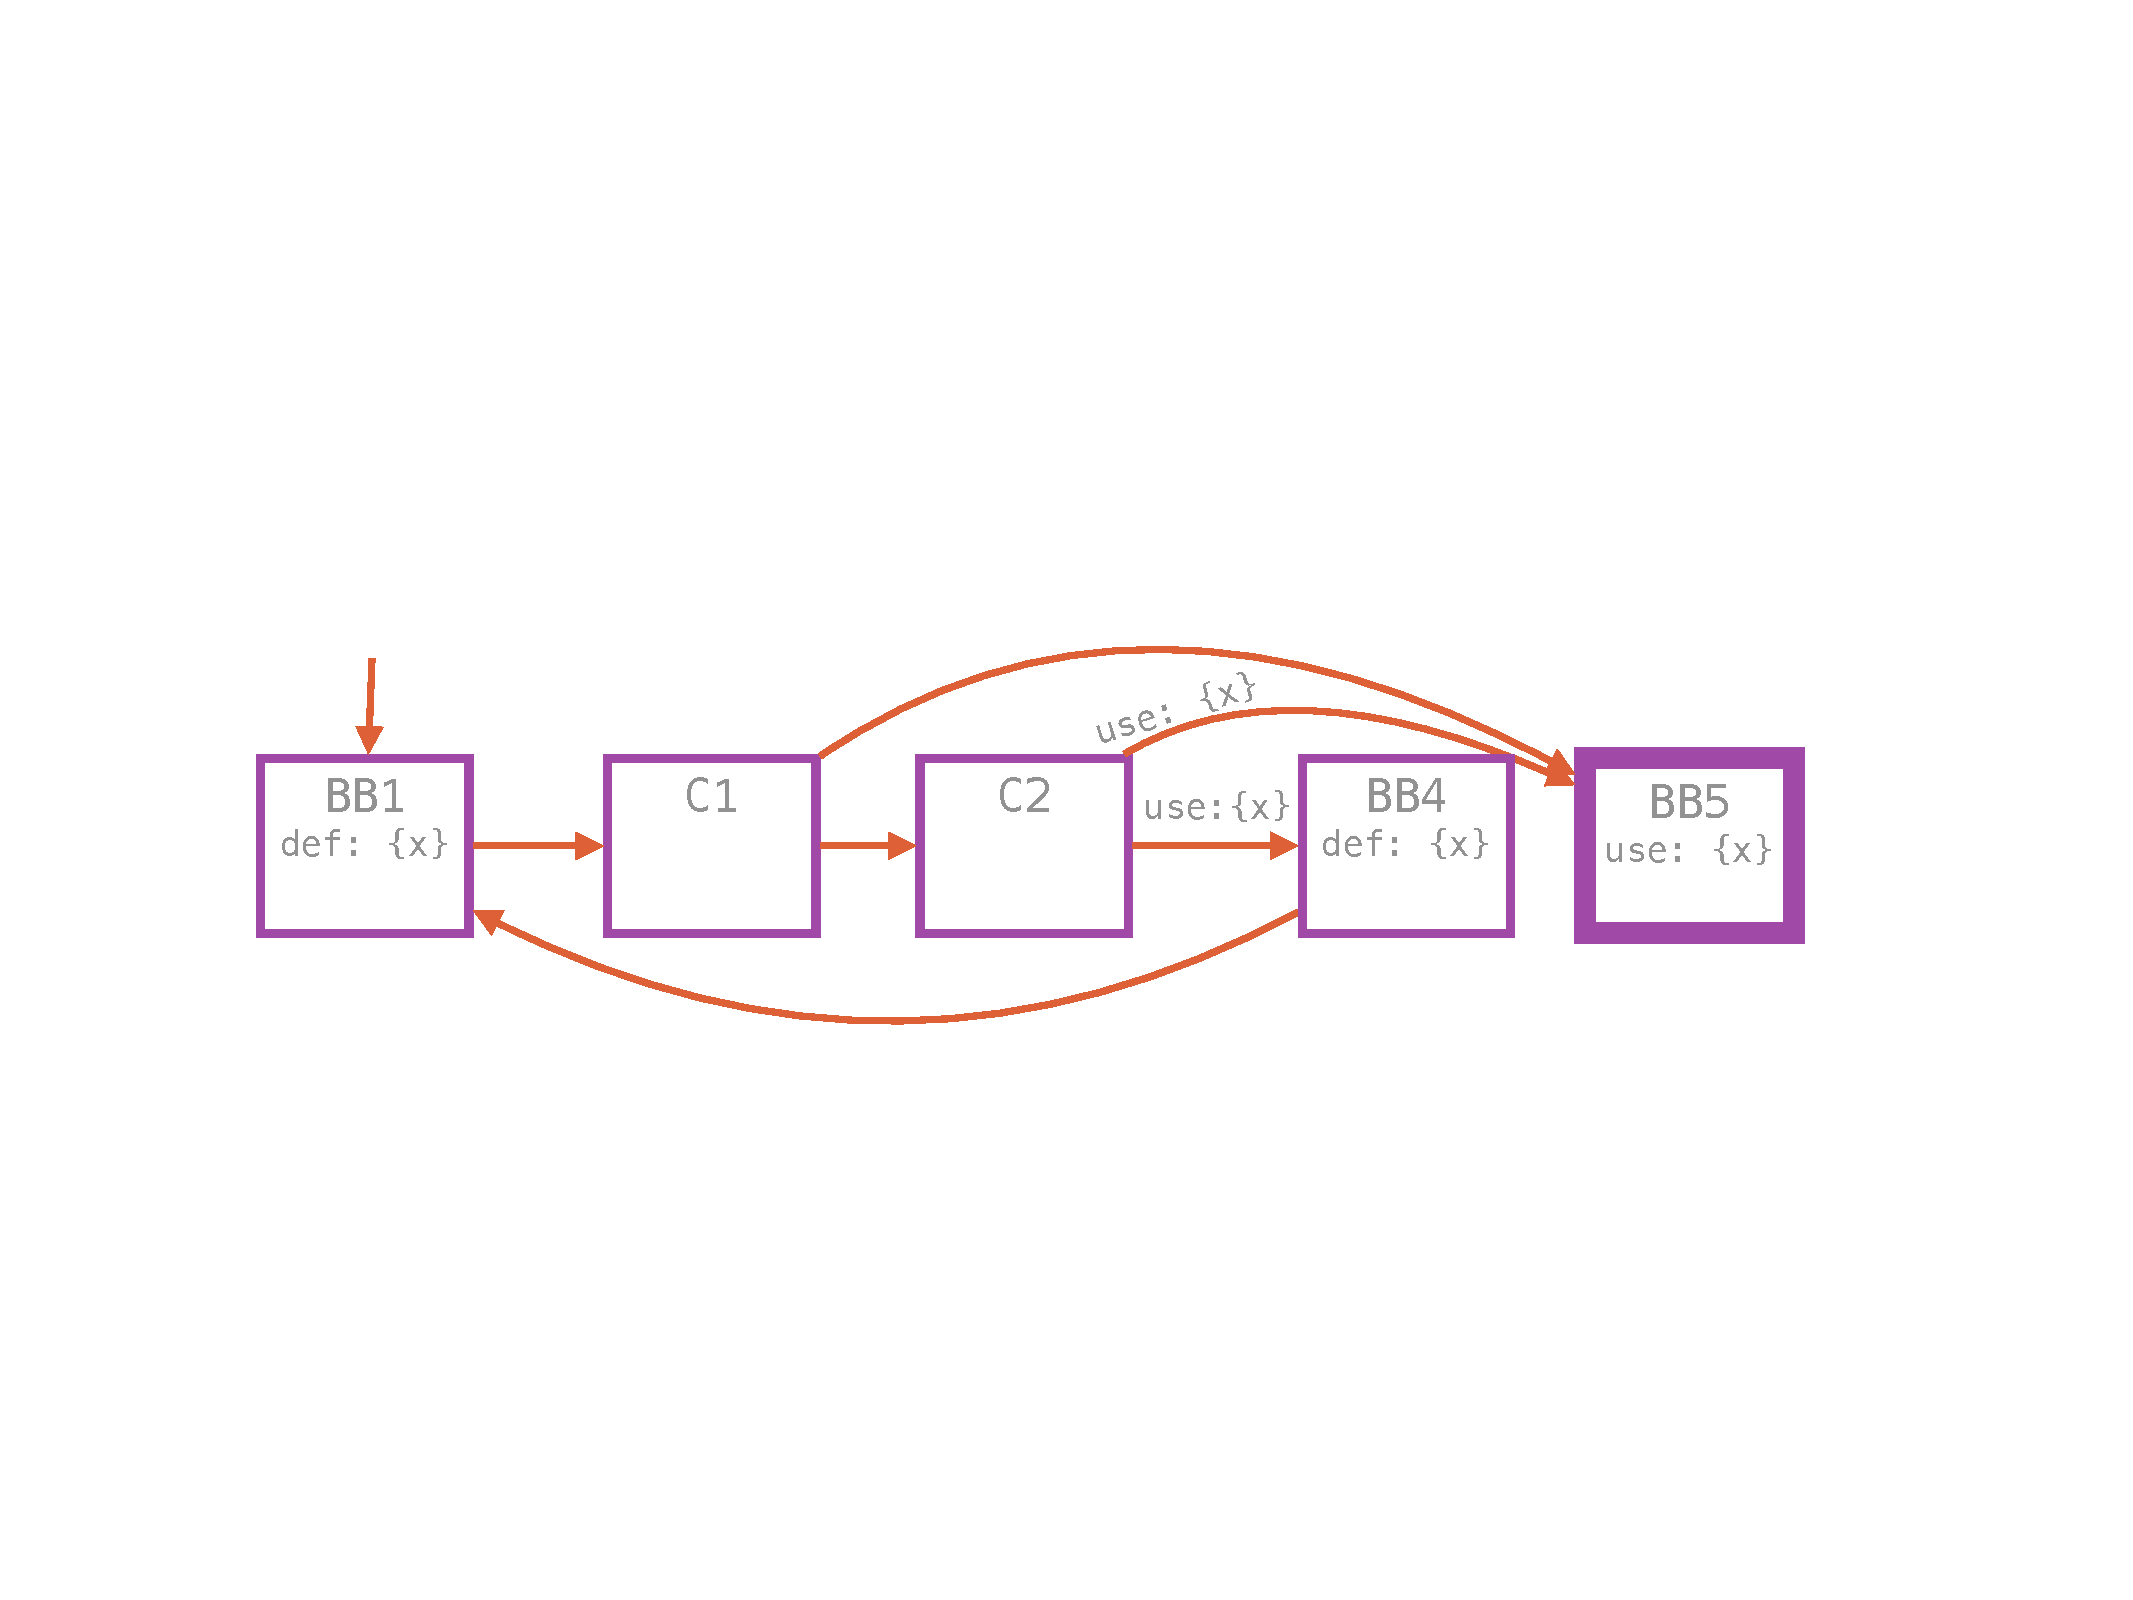
\includegraphics[width=.5\linewidth]{figures/sample-midterm-cfg}
    \end{center}
\end{figure}

\begin{parts}
\part[3] List the test requirement set of all-defs coverage with
  respect to \Code{x}. %
  \answerspace{12} %
  \begin{solution}
    The test set needs to include a test case corresponding to a test path
    that tours one of [BB1, C1, BB5], [BB1, C1, C2, BB4], or [BB1, C1,
    C2, BB5]. Note that the du-path [BB1, C1, C2, BB5] corresponds to
    two distinct du-pairs: du(BB1, BB5, x) and du(BB1, (C2, BB5), x).
  \end{solution}

\part[3] List the test requirement set of all-uses coverage with
  respect to \Code{x}. %
  \answerspace{12} %
  \begin{solution}
    The test set needs to include a test case that tours either [BB1,
    C1, BB5] or [BB1, C1, C2, BB5], a test case that tours [BB1, C1,
    C2, BB4], and a test case that tours [BB1, C1, C2, BB5]. Note
    again the overlap between the requirements generated by du(BB1,
    BB5, x) and du(BB1, (C2, BB5), x): we can satisfy all-use coverage
    with just two test cases.
  \end{solution}

\part[4] List the test requirement set of all-du-paths coverage with
  respect to \Code{x}. %
  \answerspace{12} %
  \begin{solution}
    The test set needs to include a test case that tours [BB1, C1,
    BB5], another that tours [BB1, C1, C2, BB5], one that tours [BB1,
    C1, C2, BB4], and a test case that tours [BB1, C1, C2, BB5]. Note
    that this forces a test to tour [BB1, C1, BB5], while all-use
    coverage allows a test set to skip that path, touring [BB1, C1,
    C2, BB5] instead.
  \end{solution}
\end{parts}

\newpage

% ========================================================
% Q8: ISP characteristics.  [sample-midterm Q8]
% ========================================================

\question[4] A tester defined three characteristics for the input
  parameter \texttt{car}: \textbf{Where Made}, \textbf{Energy Source},
  and \textbf{Size}. The following partitioning for these
  characteristics has (at least) two mistakes. How would you correct
  them?

  \begin{center}
  \begin{tabular}{|c|c|c|}
    \hline
    \multicolumn{3}{|c|}{\textbf{Where Made}} \\\hline
    North America & Europe & Asia \\\hline
    \multicolumn{3}{|c|}{\textbf{Energy Source}} \\\hline
    gas & electric & hybrid \\\hline
    \multicolumn{3}{|c|}{\textbf{Size}}\\\hline
    2-door & 4-door & hatchback\\\hline
  \end{tabular}
\end{center}
\answerspace{15}
\begin{solution}
  Some potential mistakes:
  \begin{itemize}
  \item \textbf{Size} describes the number of doors rather than size,
    and the categories are not \emph{disjoint}: a hatchback can have
    four doors. Divide it into proper, distinct size categories:
    [compact $|$ mid-size $|$ full-size $|$ SUV/truck].
  \item \textbf{Where Made} is not \emph{complete}: Brazil is a major
    car manufacturer, and Australia has been known to produce cars.
    Add categories, e.g.\ [North America $|$ Asia $|$ Europe $|$
    South America $|$ Other].
  \end{itemize}
  Note that each mistake violates one of the two properties a
  partition must have. Naming which property each change repairs is
  the point of the question.
\end{solution}

\newpage

% ========================================================
% Q9: logic coverage.  [sample-final Q1]
% ========================================================

\question Consider the following predicate (call it $\phi$):
  \Code{(x <= len(a) and not b) or x != y}
  \begin{parts}

\part[2] Write down the truth table for this predicate. %
  \answerspace{6} %
  \begin{solution}
    \begin{minipage}{.9\linewidth}
      \renewcommand{\arraystretch}{1.3}
      \begin{tabular}{|| c | c c c | p{1cm}||}
        \hline
        & \Code{x <= len(a)} & \Code{b} & \Code{x != y} & $\phi$ \\ [0.5ex]
        \hline\hline
        1 & T & T & T & T \\ \hline
        2 & T & T & F & F \\ \hline
        3 & T & F & T & T \\ \hline
        4 & T & F & F & T \\ \hline
        5 & F & T & T & T \\ \hline
        6 & F & T & F & F \\ \hline
        7 & F & F & T & T \\ \hline
        8 & F & F & F & F \\ [1ex] \hline
      \end{tabular}
    \end{minipage}
  \end{solution}

\part[1] Provide a minimal set of test inputs to \Code{x}, \Code{a},
  \Code{b}, and \Code{y} that satisfy predicate coverage for $\phi$.
  If this is not possible, explain why. Write your test cases in the
  form \ACC{x}{a}{b}{y}. %
  \answerspace{6} %
  \begin{solution}
    Example: \\
    \{\ACC{3}{[1,2,3,4]}{True}{4}, \ACC{3}{[1,2,3,4]}{True}{3}\}
  \end{solution}

\part[2] Provide a minimal set of test inputs that satisfy clause
  coverage for $\phi$. If this is not possible, explain why. %
  \answerspace{5} %
  \begin{solution}
    Example: \\
    \{\ACC{3}{[1,2,3,4]}{True}{4}, \ACC{10}{[1,2,3,4]}{False}{10}\}
  \end{solution}

\newpage

\part[3] Provide a formula that captures precisely the truth
  assignments where the clause \Code{x <= len(a)} determines $\phi$,
  i.e., any satisfying assignment to this formula is also a assignment
  where \Code{x <= len(a)} determines $\phi$. %
  \answerspace{4} %
  \begin{solution}
    \Code{not b and x == y} \\
    (Rows 4 and 8)
  \end{solution}

\part[3] Provide a similar formula for the clause \Code{b}. %
  \answerspace{4} %
  \begin{solution}
    \Code{x <= len(a) and x == y} \\
    (Rows 2 and 4.)
  \end{solution}

\part[3] Provide a similar formula for the clause \Code{x != y}. %
  \answerspace{4} %
  \begin{solution}
    \Code{not (x <= len(a)) or b} \\
    (Rows 1, 2, 5, 6, 7 and 8.)
  \end{solution}

\newpage

\part[4] Provide a minimal set of test inputs that satisfy Restricted
  Active Clause Coverage (RACC) for $\phi$. If this is not possible,
  explain why. Write your test cases in the form \ACC{x}{a}{b}{y}. %
  \answerspace{11} %
  \begin{solution}
    Example: \{ \\
    \ACC{0}{[1,2]}{False}{0},  \% row 4 \\
    \ACC{2}{[2]}{False}{2},    \% row 8 \\
    \ACC{2}{[1]}{False}{1},    \% row 7 \\
    \ACC{0}{[1,2]}{True}{0}    \% row 2 \\
    \}

    Rows 4/8 give RACC for \Code{x <= len(a)}, rows 2/4 for \Code{b},
    and rows 7/8 for \Code{x != y}. In each pair the minor clauses are
    unchanged.
  \end{solution}

\part[4] Provide a minimal set of test inputs that satisfy Correlated
  Active Clause Coverage (CACC) for $\phi$. Write your test cases in
  the form \ACC{x}{a}{b}{y}. If this is not possible, explain why. %
  \answerspace{11} %
  \begin{solution}
    Example: \{ \\
    \ACC{0}{[1,2]}{False}{0}, \ACC{2}{[3,5,6]}{True}{2}, \\
    \ACC{5}{[1,2,6]}{True}{3}, \ACC{5}{[1,2,3]}{False}{5} \\
    \}

    \textbf{Note 1:} this set does \emph{not} satisfy RACC, because
    \Code{x != y} only determines $\phi$ in the last three tests, and
    none of the three agrees with any of the others on the truth value
    of the two other clauses. \\
    \textbf{Note 2:} the answer to the previous part would also work
    here. Why?
  \end{solution}

\part[4] Provide a minimal set of test inputs that satisfy General
  Active Clause Coverage (GACC) for $\phi$. Write your test cases in
  the form \ACC{x}{a}{b}{y}.  If this is not possible, explain why. %
  \answerspace{11} %
  \begin{solution}
    The RACC set above also works, since RACC subsumes GACC.

    \textbf{Note:} we cannot produce a set that satisfies GACC but
    \emph{not} CACC here. In every assignment where \Code{x != y}
    determines $\phi$, $\phi$ has the same truth value as
    \Code{x != y}; the same holds for the other two clauses. So any
    pair of tests that makes a clause take both values while
    determining $\phi$ also makes $\phi$ take both values.
  \end{solution}

\end{parts}

\newpage

% ========================================================
% Q10: counting ACC requirements.  [sample-final Q2]
% ========================================================

\question[3] Suppose we have a predicate with $n$ clauses. What is the
  minimum number of test cases a test set \textbf{must} contain in
  order to provide 100\% RACC for this predicate? What about CACC and
  GACC? Explain your answer. %
  \answerspace{18} %
  \begin{solution}
    \begin{itemize}
    \item \textbf{RACC:} $n + 1$.
    \item \textbf{CACC:} 3. Consider
      $p = c_1 \oplus c_2 \oplus \ldots \oplus c_n$. Every clause
      determines $p$ under every assignment, since flipping any clause
      flips $p$. When $n$ is odd, the all-true and all-false tests
      suffice: each clause takes both values, determines $p$ in both,
      and $p$ differs between them --- so 2 tests. When $n$ is even
      the all-true and all-false tests give $p$ the same value, so a
      third test is needed.
    \item \textbf{GACC:} 2. CACC subsumes GACC, so the minimum is at
      most 3; and it is at least 2, since each clause needs one test
      where it is true and one where it is false. The two-test set
      above achieves GACC for either parity of $n$ --- under GACC we
      do not care that $p$ takes the same value in both.
    \end{itemize}
  \end{solution}

\newpage

% ========================================================
% Q11: mutation testing.  NEW --- neither practice exam covered it.
% ========================================================

\question Consider the following Python function, which adds a bonus to
  a score, caps the result at 100, and reports whether it is a pass.
  \begin{minted}{python}
def grade(score: int, bonus: int) -> str:
    total = score + bonus
    if total > 100:
        total = 100
    if total >= 60:
        return "pass"
    return "fail"
\end{minted}

  Consider the following three categories of mutation operators:
  \begin{description}
  \item[Conditionals Boundary] replace a relational operator with its
    boundary variant (\Code{>} $\leftrightarrow$ \Code{>=},
    \Code{<} $\leftrightarrow$ \Code{<=})
  \item[Math] replace one arithmetic operator with another
  \item[Inline Constant] replace a numeric literal with a different one
  \end{description}

\begin{parts}

\part[6] Using these operators, give \textbf{three} distinct
  first-order mutants of \Code{grade}, each using a different
  operator. For each, give a test case that kills it and state the
  result produced by both the original and the mutant. %
  \answerspace{20} %
  \begin{solution}
    Many correct answers. For example:
    \begin{itemize}
    \item \textbf{Boundary}, line 5: \Code{total >= 60} $\to$
      \Code{total > 60}. Killed by \Code{grade(1, 59)}: the original
      returns \Code{"pass"}, the mutant \Code{"fail"}.
    \item \textbf{Math}, line 2: \Code{score + bonus} $\to$
      \Code{score - bonus}. Killed by \Code{grade(1, 59)}:
      \Code{"pass"} vs.\ \Code{"fail"}.
    \item \textbf{Inline Constant}, line 5: \Code{60} $\to$ \Code{6}.
      Killed by \Code{grade(0, 10)}: \Code{"fail"} vs.\
      \Code{"pass"}.
    \end{itemize}
  \end{solution}

\newpage

\part[6] There is a first-order mutant of \Code{grade} that can be
  constructed using one of the three operators above and that
  \textbf{cannot} be killed. Give it, and explain why it cannot be
  killed. %
  \answerspace{20} %
  \begin{solution}
    Line 3: \Code{total > 100} $\to$ \Code{total >= 100}. The two
    versions take different branches only when
    \Code{total == 100}, and in that case the mutant executes
    \Code{total = 100}, which leaves \Code{total} unchanged. Every
    other input follows an identical path and computes an identical
    value, so no input distinguishes the mutant from the original ---
    it is an \textbf{equivalent mutant}.
  \end{solution}

\part[4] Suppose a tool generates 10 mutants of \Code{grade} and your
  test suite kills 7 of them. On inspection, 2 of the 3 survivors turn
  out to be equivalent. What \textbf{kill rate} and \textbf{mutation
    score} would you report?  What should you do with the remaining
  survivor? %
  \answerspace{18} %
  \begin{solution}
    The raw kill rate is $7/10 = 70\%$. Since equivalent mutants can
    never be killed, the mutation score discounts them:
    $7/8 = 87.5\%$.

    The remaining survivor is a \emph{killable} mutant that your suite
    does not detect. This is the key result of this mutation testing
    run, as it represents a test case that is missing from your test
    set. The right response is to write a test that kills it.
  \end{solution}

\newpage

\part[4] Why can a tool not simply discard the equivalent mutants
  before reporting a kill rate? %
  \answerspace{18} %
  \begin{solution}
    Deciding whether two programs are semantically equivalent is
    undecidable in general, so no algorithm can identify every
    equivalent mutant. Tools can use heuristics and conservative
    checks, but surviving mutants ultimately have to be triaged by
    hand. This is a significant part of the cost of mutation testing,
    and why a kill rate of 100\% is usually unattainable.
  \end{solution}

\part[4] Using the RIPR model, explain why a test case that
  \emph{executes} a mutated statement may nonetheless fail to kill the
  mutant. Give a concrete example using \Code{grade}. %
  \answerspace{20} %
  \begin{solution}
    Executing the mutated statement establishes only
    \emph{reachability}. The mutant is killed only if the mutation
    also makes the program state differ (\emph{infection}) and that
    difference reaches an output the test checks
    (\emph{propagation}).

    Example: mutate line 4 to \Code{total = 99}. The test
    \Code{grade(200, 0)} reaches and executes the mutated line, and
    the state \emph{is} infected --- \Code{total} is 99 rather than
    100 --- but both values are at least 60, so both versions return
    \Code{"pass"} and the difference never propagates to the output.
  \end{solution}

\end{parts}

\newpage
\begin{center}
  [EMPTY PAGE 1]
\end{center}

\newpage
\begin{center}
  [EMPTY PAGE 2]
\end{center}

\end{questions}

\end{document}
